% BEGIN TEMPLATE
\documentclass{article}
\usepackage{graphicx}
\usepackage{hyperref} 
\usepackage{xcolor}
\usepackage{nameref}
\usepackage{listings}
\usepackage{float}
\usepackage[title]{appendix}
\usepackage[ruled]{algorithm2e}
\graphicspath{ {../../images/} }
\bibliographystyle{acm}
% CHANGE THESE
\newcommand{\courseListing}{CSCI 8920}
\newcommand{\courseName}{Fundamentals of Deep Learning}
\newcommand{\assignmentTitle}{Homework Assignment \#3}
\newcommand{\assignmentSubtitle}{LeNet, MobileNet, and Error Modeling}
\usepackage{geometry}
\geometry{margin=1in}

\hypersetup{
    colorlinks,
    linkcolor={red!50!black},
    citecolor={blue!50!black},
    urlcolor={blue!80!black}
}
\urlstyle{same}
\definecolor{codegreen}{rgb}{0,0.6,0}
\definecolor{codegray}{rgb}{0.5,0.5,0.5}
\definecolor{codepurple}{rgb}{0.58,0,0.82}
\lstdefinestyle{mystyle}{
    commentstyle=\color{codegreen},
    keywordstyle=\color{magenta},
    numberstyle=\tiny\color{codegray},
    stringstyle=\color{codepurple},
    basicstyle=\ttfamily\footnotesize,
    breakatwhitespace=false,         
    breaklines=true,                 
    captionpos=b,                    
    keepspaces=true,                 
    numbers=left,                    
    numbersep=5pt,                  
    showspaces=false,                
    showstringspaces=false,
    showtabs=false,                  
    tabsize=2
}

\lstset{style=mystyle}

\begin{document}
  \begin{center}
  
\includegraphics[scale=0.15]{UNO-Logo-Color.png}
  \\[0.3in]
  \textbf{\courseListing{}}\\
  \courseName{}
  \\[0.75in]
  \textbf{\assignmentTitle{}}\\
  \assignmentSubtitle{}
  \\[0.75in]
  \textbf{Patrick Davlin}
  \\[0.75in]
  \textbf{Computer Science Department}\\
  \textbf{Peter Kiewit Institute}\\
  \textbf{University of Nebraska}
  \\[0.75in]
  \textbf{Spring 2021}
  \\[0.3in]
  
\includegraphics[scale=0.075]{UNO-Icon-Color.png}
  \newpage
\end{center}
  \graphicspath{{./images/}}
% END TEMPLATE

\section{Project Setup} \label{setup}
Similarly to Assignment #1 and #2, this assignment was done entirely on a local machine using the following specific packages:
\begin{itemize}
    \item Python 3.8.6 
    \item Tensorflow 2.4.1
    \item Matplotlib 3.3.4
\end{itemize}.

There is little else to say about the setup--with the Tensorflow tooling configured there is relatively little variation from assignment to assignment. 

\section{Implementation} \label{impl}
\textit{Note: this section discusses sections of code; the entire project can be found in the \nameref{codelist}}.
\subsection{Loading MNIST Data}
The first task for the assignment was to load and output MNIST data:
\begin{lstlisting}[language=Python]
# Load CIFAR10 data
(x_train, y_train), (x_test, y_test) = mnist.load_data()

# convert from uint to floats, and normalize to [0,1]
x_train = x_train.astype('float32')
x_test = x_test.astype('float32')
x_train = x_train / 255
x_test = x_test / 255

x_train = x_train.reshape(x_train.shape[0], 28, 28, 1)
x_test = x_test.reshape(x_test.shape[0], 28, 28, 1)

y_train = to_categorical(y_train, 10)
y_test = to_categorical(y_test, 10)


print('x_train.shape = ', x_train.shape, ' y_train.shape = ', y_train.shape)
print('x_test.shape = ', x_test.shape, ' y_test.shape = ', y_test.shape)

print('data type: ', type(x_train[0][0][0]))
print('label type: ', type(y_train[0][0]))

# plt.imshow(x_train[0], cmap='Greys')
plot_images(x_train)

# x_train = np.expand_dims(x_train, axis=-1)
\end{lstlisting}
To confirm, the resulting images are below:

\begin{figure}[H]
    \centering
    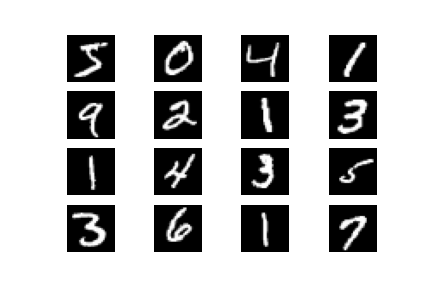
\includegraphics[width=3in]{csci-8920/hw-2/images/mnist.png}
    \caption{MNIST images}
    \label{fig:mnist}
\end{figure}

\subsection{LeNet Model}
The LeNet 5 implementation was carried forward from Assignment #2.
This implementation makes use of the functional Keras construction, where the model is compiled as a function of inputs (the MNIST image data) and outputs (the result of a series of layer operations upon those inputs), as shown below:
\begin{lstlisting}[language=Python]
def LeNet_impl():

  data_in = keras.Input(shape=(28,28,1))
  kernel_size=(5,5)

  x = Conv2D(6, kernel_size, activation='relu', strides = (1,1), input_shape= (28,28,1), padding='same')(data_in)
  x = AveragePooling2D(pool_size=(2,2), strides = (2,2))(x)
  x = Conv2D(16, kernel_size, activation='relu', strides = (1,1))(x)
  x = AveragePooling2D(pool_size=(2,2), strides = (2,2))(x)
  x = Conv2D(120, kernel_size, activation='relu', strides = (1,1))(x)
  x = Flatten()(x)
  x = Dense(120, activation='relu')(x)
  x = Dense(84, activation='relu')(x)
  x = Dropout(0.5)(x)
  x = Dense(10, activation='softmax')(x)
  lenet_model = keras.Model(inputs = data_in, outputs = x, name = "lenet_model")
  lenet_model.compile(optimizer = 'SGD', loss = keras.losses.categorical_crossentropy, metrics = ['accuracy'])
  lenet_model.summary()
  return lenet_model
\end{lstlisting}

The \lstinline{model.summary()} result is shown below:

\begin{lstlisting}
Model: "lenet_model"
_________________________________________________________________
Layer (type)                 Output Shape              Param #   
=================================================================
input_1 (InputLayer)         [(None, 28, 28, 1)]       0         
_________________________________________________________________
conv2d (Conv2D)              (None, 28, 28, 6)         156       
_________________________________________________________________
average_pooling2d (AveragePo (None, 14, 14, 6)         0         
_________________________________________________________________
conv2d_1 (Conv2D)            (None, 10, 10, 16)        2416      
_________________________________________________________________
average_pooling2d_1 (Average (None, 5, 5, 16)          0         
_________________________________________________________________
conv2d_2 (Conv2D)            (None, 1, 1, 120)         48120     
_________________________________________________________________
flatten (Flatten)            (None, 120)               0         
_________________________________________________________________
dense (Dense)                (None, 120)               14520     
_________________________________________________________________
dense_1 (Dense)              (None, 84)                10164     
_________________________________________________________________
dropout (Dropout)            (None, 84)                0         
_________________________________________________________________
dense_2 (Dense)              (None, 10)                850       
=================================================================
Total params: 76,226
Trainable params: 76,226
Non-trainable params: 0
_________________________________________________________________
\end{lstlisting}

\\The model is then trained against the input MNIST data using the \lstinline{model.fit()} command as shown below:

\begin{lstlisting}[language=Python]
# default model run/train
model_default = LeNet_impl()
default_fitness = model_default.fit(x=x_train, y=y_train, steps_per_epoch=128, epochs=500, verbose=1, validation_data=(x_test, y_test))
model_default.save('./models/default')
with open('./histories/default/default.txt', 'w') as default_history_file:
    default_history_file.write(json.dumps(default_fitness.history))
\end{lstlisting}

For 500 epochs, as shown in this code, the results of the training can be visualized:

\begin{figure}[H]
\centering
\begin{subfigure}
  \centering
  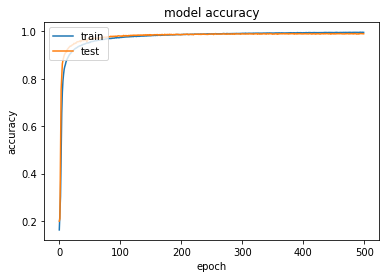
\includegraphics[width=3in]{csci-8920/hw-2/images/accuracy.png}
  \label{fig:accuracy}
\end{subfigure}%
\begin{subfigure}
  \centering
  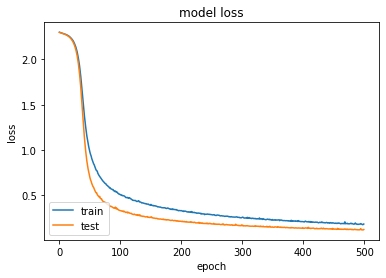
\includegraphics[width=3in]{csci-8920/hw-2/images/loss.png}
  \label{fig:loss}
\end{subfigure}
\caption{Results of LeNet 5 model after 500 epochs.}
\label{fig:default}
\end{figure}

From the outset it's obvious that 500 epochs with a batch size of 128 is much too high.
The model appears to stabilize before the 50th epoch.
The model can be re-run accordingly:

\begin{figure}[H]
\centering
\begin{subfigure}
  \centering
  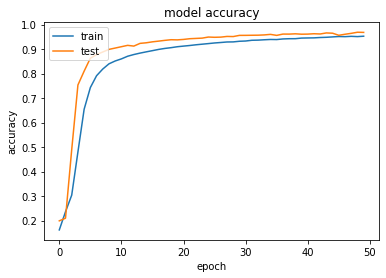
\includegraphics[width=3in]{csci-8920/hw-2/images/accuracy-50.png}
  \label{fig:accuracy-50}
\end{subfigure}%
\begin{subfigure}
  \centering
  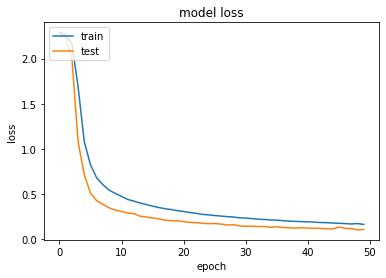
\includegraphics[width=3in]{csci-8920/hw-2/images/loss-50.png}
  \label{fig:loss-50}
\end{subfigure}
\caption{Results of LeNet 5 model after 50 epochs.}
\label{fig:default-50}
\end{figure}

Complete output supporting this is available in the \nameref{completeout} Appendix.

\subsection{MobileNet Model}
In addition to the LeNet model from Assignment 2, a new MobileNet model was implemented for this assignment.
The functional implementation is shown below:

\begin{lstlisting}[language=Python]
def MobileNet_impl(alpha = 1):
  data_in = Input(shape = (28, 28, 1))
  x = ZeroPadding2D(padding = (2, 2))(data_in)

  x = Conv2D(int(32 * alpha), (3, 3), padding = 'same')(x)
  x = BatchNormalization()(x)
  x = Activation('relu')(x)
  x = depthwise_sep_conv(x, 64, alpha)
  x = depthwise_sep_conv(x, 128, alpha, strides= (2, 2))
  x = depthwise_sep_conv(x, 128, alpha)
  x = depthwise_sep_conv(x, 256, alpha, strides= (2, 2))
  x = depthwise_sep_conv(x, 256, alpha)
  x = depthwise_sep_conv(x, 512, alpha, strides= (2, 2))
  for _ in range(5):
    x = depthwise_sep_conv(x, 512, alpha)
  x = depthwise_sep_conv(x, 1024, alpha, strides= (2, 2))
  x = depthwise_sep_conv(x, 1024, alpha)
  x = GlobalAveragePooling2D()(x)
  x = Dense(units = 10)(x)
  x = Activation('softmax')(x)

  mobilenet_model = keras.Model(inputs = data_in, outputs = x, name = "mobilenet_model")
  mobilenet_model.compile(optimizer = optimizers.RMSprop(lr = 0.01), loss = keras.losses.categorical_crossentropy, metrics = ['accuracy'])
  return mobilenet_model
\end{lstlisting}

This model makes use of a function which applies several layers in a loop, shown below:

\begin{lstlisting}[language=Python]
def depthwise_sep_conv(x, filters, alpha, strides = (1, 1)):
    y = DepthwiseConv2D((3, 3), padding = 'same', strides = strides)(x)
    y = BatchNormalization()(y)
    y = Activation('relu')(y)
    y = Conv2D(int(filters * alpha), (1, 1), padding = 'same')(y)
    y = BatchNormalization()(y)
    y = Activation('relu')(y)
    return y
\end{lstlisting}

\begin{figure}[H]
\centering
\begin{subfigure}
  \centering
  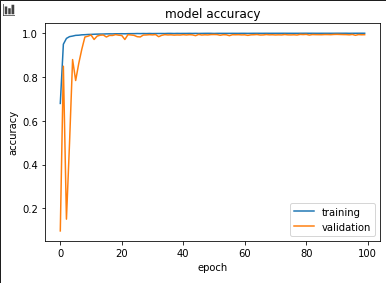
\includegraphics[width=3in]{csci-8920/hw-3/images/mnet_100_epoch.png}
  \label{fig:m-accuracy}
\end{subfigure}%
\begin{subfigure}
  \centering
  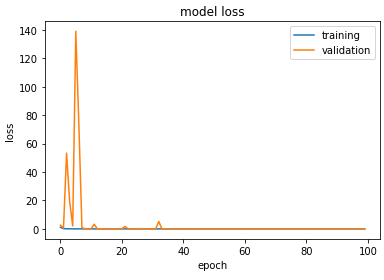
\includegraphics[width=3in]{csci-8920/hw-3/images/mnet_loss_100.png}
  \label{fig:m-loss}
\end{subfigure}
\caption{Results of MobileNet model after 500 epochs.}
\label{fig:m-default}
\end{figure}

The model appears to stabilize before the 15th epoch:

\begin{figure}[H]
\centering
\begin{subfigure}
  \centering
  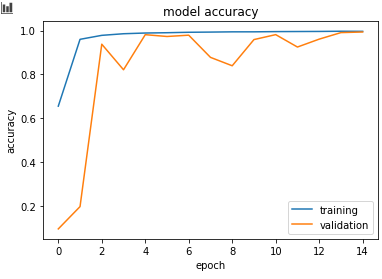
\includegraphics[width=3in]{csci-8920/hw-3/images/mnet_15_epoch.png}
  \label{fig:accuracy-15}
\end{subfigure}%
\begin{subfigure}
  \centering
  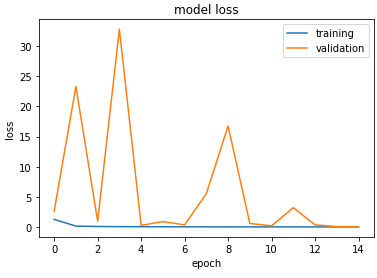
\includegraphics[width=3in]{csci-8920/hw-3/images/mnet_loss_15.png}
  \label{fig:loss-15}
\end{subfigure}
\caption{Results of MobileNet model after 15 epochs.}
\label{fig:default-15}
\end{figure}

The \lstinline{model.summary()} results are shown in the \nameref{msum} Appendix.

\subsection{Error Surface Modeling 1}

The equation implemented for this section is as follows:

\begin{equation}
    J(\theta) = (1-\alpha) \theta_0 + \alpha \times \theta_1
\end{equation}

To do this in code, weights from an untrained model and a fully trained model were combined in a new, blank model.
The combined model was then scored with \lstinline{.evaluate()} against validation MNIST data:

\begin{lstlisting}[language=Python]
def combine_models(alpha, theta_0_model, theta_star_model, new_model):
    for index, weights in enumerate(theta_0_model.trainable_weights):
        new_model.trainable_weights[index].assign((1 - alpha) * weights)

    print(len(theta_star_model.trainable_weights))
    for index, weights in enumerate(theta_star_model.trainable_weights):
        new_model.trainable_weights[index].assign_add(alpha * weights)
    return new_model
\end{lstlisting}

This worked fine for LeNet, but for some reason led to nearly-infinite values between $\alpha = 1$ and $\alpha = 2$ for MobileNet, as shown below:

\begin{figure}[H]
\centering
\begin{subfigure}
  \centering
  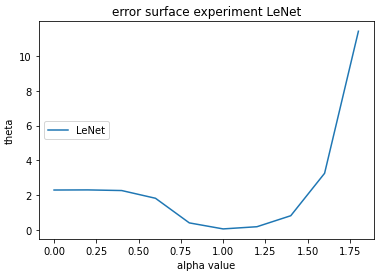
\includegraphics[width=3in]{csci-8920/hw-3/images/theta_lenet.png}
  \label{fig:ln-2}
\end{subfigure}%
\begin{subfigure}
  \centering
  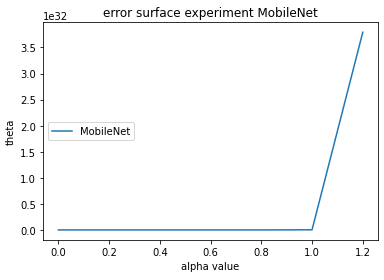
\includegraphics[width=3in]{csci-8920/hw-3/images/theta_mobilenet.png}
  \label{fig:mn-2}
\end{subfigure}
\caption{Results of Error Surface Experiment 1.}
\label{fig:default-15}
\end{figure}

\subsection{Error Surface Modeling 2}
The second exercise was much more difficult.
Finding information about the expectations for the desired graph, and for PCA modeling in general, proved to be a difficult task.
To obtain results, each model needed a variation on this callback to record weights after each epoch for a layer in the model:

\begin{lstlisting}[language=Python]
mobilenet_weights_dict = {}

mobilenet_1 = MobileNet_impl()
mobilenet_weight_callback = tf.keras.callbacks.LambdaCallback( on_epoch_end=lambda epoch, logs: mobilenet_weights_dict.update({epoch:mobilenet_1.layers[2].get_weights()}))
mobilenet_fitness = mobilenet_1.fit(x=x_train, y=y_train, steps_per_epoch=128, epochs=15, verbose=1, validation_data=(x_test, y_test), callbacks=mobilenet_weight_callback)
\end{lstlisting}

Results of PCA were applied on the collected weights as follows:

\begin{lstlisting}[language=Python]
pca_w = []
for epoch, weights in mobilenet_weights_dict.items():
    print("weights at 2nd layer for epoch {}: {}".format(epoch, weights))
    pca_w.append([weights[0][0][0][0], weights[1]])

variance_x = []
variance_y = []
for w in pca_w:
    pca = PCA(n_components=2)
    pca.fit_transform(w)
    variance.append(pca.explained_variance_)


print("varience len: ", len(variance))
for v in range(len(variance)):
    variance_x.append(variance[v][0])
    variance_y.append(variance[v][1])
\end{lstlisting}

The variancy values were, finally, plotted:

\begin{figure}[H]
\centering
\begin{subfigure}
  \centering
  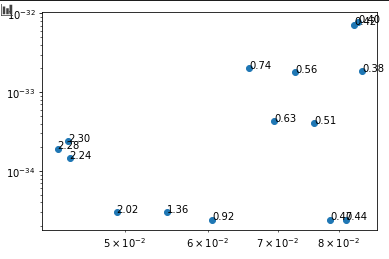
\includegraphics[width=3in]{csci-8920/hw-3/images/lenet_final.png}
  \label{fig:ln-2}
\end{subfigure}%
\begin{subfigure}
  \centering
  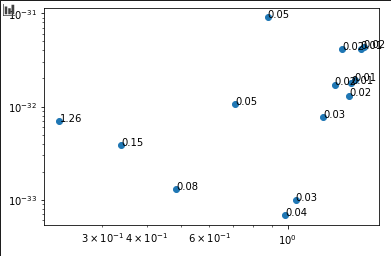
\includegraphics[width=3in]{csci-8920/hw-3/images/mobilenet_final.png}
  \label{fig:mn-2}
\end{subfigure}
\caption{Results of Error Surface Experiment 2. Left is LeNet, Right is MobileNet.}
\label{fig:default-15}
\end{figure}

\section{Conclusions}
The experiments run in the course of this assignment were valuable in encouraging more careful thought about the layers that compose Keras models.
This was a difficult and somewhat unclear assignment, because understanding the variance and error rates is a conceptually challenging task.
A lot of confusion was encountered in attempting to apply these concepts.
Moreover, this assignment was due the same week as a major project for another class, which left relatively less time to work on it relative to other, prior assignments in the course.

\newpage
\begin{appendices}
\section{MobileNet Model Summary} \label{msum}
\begin{lstlisting}
Model: "mobilenet_model"
_________________________________________________________________
Layer (type)                 Output Shape              Param #   
=================================================================
input_34 (InputLayer)        [(None, 28, 28, 1)]       0         
_________________________________________________________________
zero_padding2d_15 (ZeroPaddi (None, 32, 32, 1)         0         
_________________________________________________________________
conv2d_264 (Conv2D)          (None, 32, 32, 32)        320       
_________________________________________________________________
batch_normalization_405 (Bat (None, 32, 32, 32)        128       
_________________________________________________________________
activation_420 (Activation)  (None, 32, 32, 32)        0         
_________________________________________________________________
depthwise_conv2d_195 (Depthw (None, 32, 32, 32)        320       
_________________________________________________________________
batch_normalization_406 (Bat (None, 32, 32, 32)        128       
_________________________________________________________________
activation_421 (Activation)  (None, 32, 32, 32)        0         
_________________________________________________________________
conv2d_265 (Conv2D)          (None, 32, 32, 64)        2112      
_________________________________________________________________
batch_normalization_407 (Bat (None, 32, 32, 64)        256       
_________________________________________________________________
activation_422 (Activation)  (None, 32, 32, 64)        0         
_________________________________________________________________
depthwise_conv2d_196 (Depthw (None, 16, 16, 64)        640       
_________________________________________________________________
batch_normalization_408 (Bat (None, 16, 16, 64)        256       
_________________________________________________________________
activation_423 (Activation)  (None, 16, 16, 64)        0         
_________________________________________________________________
conv2d_266 (Conv2D)          (None, 16, 16, 128)       8320      
_________________________________________________________________
batch_normalization_409 (Bat (None, 16, 16, 128)       512       
_________________________________________________________________
activation_424 (Activation)  (None, 16, 16, 128)       0         
_________________________________________________________________
depthwise_conv2d_197 (Depthw (None, 16, 16, 128)       1280      
_________________________________________________________________
batch_normalization_410 (Bat (None, 16, 16, 128)       512       
_________________________________________________________________
activation_425 (Activation)  (None, 16, 16, 128)       0         
_________________________________________________________________
conv2d_267 (Conv2D)          (None, 16, 16, 128)       16512     
_________________________________________________________________
batch_normalization_411 (Bat (None, 16, 16, 128)       512       
_________________________________________________________________
activation_426 (Activation)  (None, 16, 16, 128)       0         
_________________________________________________________________
depthwise_conv2d_198 (Depthw (None, 8, 8, 128)         1280      
_________________________________________________________________
batch_normalization_412 (Bat (None, 8, 8, 128)         512       
_________________________________________________________________
activation_427 (Activation)  (None, 8, 8, 128)         0         
_________________________________________________________________
conv2d_268 (Conv2D)          (None, 8, 8, 256)         33024     
_________________________________________________________________
batch_normalization_413 (Bat (None, 8, 8, 256)         1024      
_________________________________________________________________
activation_428 (Activation)  (None, 8, 8, 256)         0         
_________________________________________________________________
depthwise_conv2d_199 (Depthw (None, 8, 8, 256)         2560      
_________________________________________________________________
batch_normalization_414 (Bat (None, 8, 8, 256)         1024      
_________________________________________________________________
activation_429 (Activation)  (None, 8, 8, 256)         0         
_________________________________________________________________
conv2d_269 (Conv2D)          (None, 8, 8, 256)         65792     
_________________________________________________________________
batch_normalization_415 (Bat (None, 8, 8, 256)         1024      
_________________________________________________________________
activation_430 (Activation)  (None, 8, 8, 256)         0         
_________________________________________________________________
depthwise_conv2d_200 (Depthw (None, 4, 4, 256)         2560      
_________________________________________________________________
batch_normalization_416 (Bat (None, 4, 4, 256)         1024      
_________________________________________________________________
activation_431 (Activation)  (None, 4, 4, 256)         0         
_________________________________________________________________
conv2d_270 (Conv2D)          (None, 4, 4, 512)         131584    
_________________________________________________________________
batch_normalization_417 (Bat (None, 4, 4, 512)         2048      
_________________________________________________________________
activation_432 (Activation)  (None, 4, 4, 512)         0         
_________________________________________________________________
depthwise_conv2d_201 (Depthw (None, 4, 4, 512)         5120      
_________________________________________________________________
batch_normalization_418 (Bat (None, 4, 4, 512)         2048      
_________________________________________________________________
activation_433 (Activation)  (None, 4, 4, 512)         0         
_________________________________________________________________
conv2d_271 (Conv2D)          (None, 4, 4, 512)         262656    
_________________________________________________________________
batch_normalization_419 (Bat (None, 4, 4, 512)         2048      
_________________________________________________________________
activation_434 (Activation)  (None, 4, 4, 512)         0         
_________________________________________________________________
depthwise_conv2d_202 (Depthw (None, 4, 4, 512)         5120      
_________________________________________________________________
batch_normalization_420 (Bat (None, 4, 4, 512)         2048      
_________________________________________________________________
activation_435 (Activation)  (None, 4, 4, 512)         0         
_________________________________________________________________
conv2d_272 (Conv2D)          (None, 4, 4, 512)         262656    
_________________________________________________________________
batch_normalization_421 (Bat (None, 4, 4, 512)         2048      
_________________________________________________________________
activation_436 (Activation)  (None, 4, 4, 512)         0         
_________________________________________________________________
depthwise_conv2d_203 (Depthw (None, 4, 4, 512)         5120      
_________________________________________________________________
batch_normalization_422 (Bat (None, 4, 4, 512)         2048      
_________________________________________________________________
activation_437 (Activation)  (None, 4, 4, 512)         0         
_________________________________________________________________
conv2d_273 (Conv2D)          (None, 4, 4, 512)         262656    
_________________________________________________________________
batch_normalization_423 (Bat (None, 4, 4, 512)         2048      
_________________________________________________________________
activation_438 (Activation)  (None, 4, 4, 512)         0         
_________________________________________________________________
depthwise_conv2d_204 (Depthw (None, 4, 4, 512)         5120      
_________________________________________________________________
batch_normalization_424 (Bat (None, 4, 4, 512)         2048      
_________________________________________________________________
activation_439 (Activation)  (None, 4, 4, 512)         0         
_________________________________________________________________
conv2d_274 (Conv2D)          (None, 4, 4, 512)         262656    
_________________________________________________________________
batch_normalization_425 (Bat (None, 4, 4, 512)         2048      
_________________________________________________________________
activation_440 (Activation)  (None, 4, 4, 512)         0         
_________________________________________________________________
depthwise_conv2d_205 (Depthw (None, 4, 4, 512)         5120      
_________________________________________________________________
batch_normalization_426 (Bat (None, 4, 4, 512)         2048      
_________________________________________________________________
activation_441 (Activation)  (None, 4, 4, 512)         0         
_________________________________________________________________
conv2d_275 (Conv2D)          (None, 4, 4, 512)         262656    
_________________________________________________________________
batch_normalization_427 (Bat (None, 4, 4, 512)         2048      
_________________________________________________________________
activation_442 (Activation)  (None, 4, 4, 512)         0         
_________________________________________________________________
depthwise_conv2d_206 (Depthw (None, 2, 2, 512)         5120      
_________________________________________________________________
batch_normalization_428 (Bat (None, 2, 2, 512)         2048      
_________________________________________________________________
activation_443 (Activation)  (None, 2, 2, 512)         0         
_________________________________________________________________
conv2d_276 (Conv2D)          (None, 2, 2, 1024)        525312    
_________________________________________________________________
batch_normalization_429 (Bat (None, 2, 2, 1024)        4096      
_________________________________________________________________
activation_444 (Activation)  (None, 2, 2, 1024)        0         
_________________________________________________________________
depthwise_conv2d_207 (Depthw (None, 2, 2, 1024)        10240     
_________________________________________________________________
batch_normalization_430 (Bat (None, 2, 2, 1024)        4096      
_________________________________________________________________
activation_445 (Activation)  (None, 2, 2, 1024)        0         
_________________________________________________________________
conv2d_277 (Conv2D)          (None, 2, 2, 1024)        1049600   
_________________________________________________________________
batch_normalization_431 (Bat (None, 2, 2, 1024)        4096      
_________________________________________________________________
activation_446 (Activation)  (None, 2, 2, 1024)        0         
_________________________________________________________________
global_average_pooling2d_15  (None, 1024)              0         
_________________________________________________________________
dense_69 (Dense)             (None, 10)                10250     
_________________________________________________________________
activation_447 (Activation)  (None, 10)                0         
=================================================================
Total params: 3,249,482
Trainable params: 3,227,594
Non-trainable params: 21,888
_________________________________________________________________
\end{lstlisting}
\section{Complete Code Listing} \label{codelist}
\lstinputlisting[language=Python]{hw-3.py}
\end{appendices}
\end{document}